\capitulo{4}{Técnicas y herramientas}

\section{Metodología Ágil Scrum}\label{scrum}
A lo largo del proyecto se intentado seguir la \textit{metodología ágil Scrum}, pero adaptada ya que para pdoer aplciar esta metodología es necesario contar con un equipo, en el cuál los diferentes miembros se reparten las roles entre los diferentes miembros que lo conforman. En este caso, lso roles recaeen todo sobre una única persona.

\imagen{scrum}{Pasos de la metodología Scrum}

En primer lugar se encuentra el \textit{Product Backlog} \cite{scrum} que se trata del alcance del proyecto, el cuál va variando dependiendo de los \textit{feedbacks} que se van obteniendo en cada \textit{sprint}.

Seguidamente, se encuentra el \textit{Sprint Backlog}, dónde se marcan los requerimientos que deben de alcanzar durante el \textit{sprint} que se va a iniciar, es decir, se trata de acortar las tareas de cada uno 
de los \textit{sprints}.

La siguiente etapa es el \textit{Sprint}, en la cuál tiene lugar la planificación, la implementación, revisión y retrospectiva de la nueva característica software.
Esta etapa suele tener una duración de una a dos semanas.

Como último paso del proceso, se enecuentra el \textit{incremento del producto}, esta fase consiste en tener una reunión con el cliente con la nueva característica en funcionamiento con el objetivo de obtener una \textit{retroalimentación} por parte del cliente y así volver a empezar el proceso de nuevo.


\section{Lenguaje de programación}
A la hora de empezar un nuevo proyecto es importante relacionado con el \textit{Machine Learning} y el \textit{Edge Computing}, es muy importante seleccionar el lenguaje, con el cuál queremos trabajar destacando dos: \textbf{Python} \cite{python} y \textbf{Matlab} \cite{matlab}.
En este caso se decantó por el uso de \textit{Python}, debido al mayor conocimiento de este lenaguaje y haber trabajado más con este lenguaje que con \textit{Matlab}.
No hay grandes ventajas entre escoger uno u otro.

\subsection{Python}
Python es un lenguaje de programación multiplataforma y multiparadigma \footnote{Debido a que soporta parcialmente la orientación a objetos, la programación funcional y la imperativa.}, destacando entre sus características la legibilidad y la limpieza del código. Python es un \textit{software open source}, siendo por ello gratuito sus uso.

Fue desarrollado al inicio de la década de los 90 por \textit{Guido van Rosseun}. Fue implementado como el sucesor del lenguaje \textit{ABC} y se encuentra fuertemente influenciado por otros como: ABC, Ada, ALGOL 68, APL, C, C++, CLU, Dylan, Haskell, Icon, Java,
Lips, Modula-3, Perl, Standard ML.

Su principal objetivo es automatizar los procesos, con el fin de minimizar tanto el tiempo de desarrollo, como complicaciones, debido a esto, hoy en día Python es uno de los lenguajes más usados para el desarrolo de todo tipo de aplicaciones.

\subsection{Tensorflow}
\textit{Tensorflow} \cite{tensorflow} es una biblioteca de código abierto, la cuál fue lanzada en el año 2015 por Google, la cuál es muy utilizada por muchas empresas resultado de gran utilidad por su versatilidad y nivel de desarrollo.

Esta herramienta se basa en el \textbf{Deep Learning,} a pesar de que el mercado habia herramientas similares como \textit{DistBelief} \cite{distBelief}, la cuál también fue construida por Google en el año 2011, como un sistema propietario de aprendizaje automático. Su uso creció rápidamente debido al uso de compaañias como \textit{Alphabet}. Pero los años pasaron y el avance de la tecnología 
hizo que las necesidades aumentasen, haciendo que Google invirtiese tiempo para mejorarla, dando lugar a la actual \textbf{Tensorflow,} una herramienta con un conjunto de datos mayor y con mayor capacidad de almacenamiento y modificación.

Se basa en un sistema de redes neuronales, lo cuál permite relacionar varios datos en la red de manera simultánea, es decir, imita lo que hace el cerebro humano.

\section{TensorRT}
\textit{TensorRT} \cite{tensorrt} es un \textit{framework} de aprendizaje automático, el cuál fue publicado por \textbf{Nvidia} para ejecutar inferencias que son interferencias de aprendizaje automático en su hardware. Este \textit{framework}, se encuentra altamente cualificado para ejecutarse en \textit{GPUs Nvidia}, siendo una de las formas más rápidas de ejecutar un modelo en este momento.

\imagen{workflowTensorrt}{Workflow del framework \textit{Tensorrt} \cite{imgTRT}}

\section{Flask}
\textit{Flask} \cite{flask} es un framework de Python, utilizado para crear aplicaciones web, APIs... En el partimos de un lienzo en blanco, es decir, partimos totalmente de cero, lo cuál nos permite utilizar sólo los módulos que necesitemos para nuestra aplicación.
Facilitando el trabajo a la hora del desarrollo, al sólo tener la necesidad de importar unicámente lo necesario al proyecto.

Con este framework se puede hacer lo mismo que con Django, siendo este más pesado y con una curva de aprendizaje muchisimo más grande que la que posee Flask, la cuál es más pequeña.

\begin{figure}[!h]
		\centering
		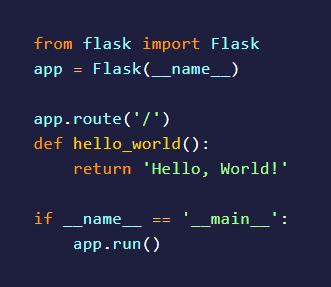
\includegraphics[width=0.4\textwidth]{holaMundoFlask}
		\caption{Hola Mundo en el framework Flask \cite{flask}}\label{fig:holaMundoFlask}
	\end{figure}
\begin{figure}[!h]
		\centering
		
\includegraphics[width=0.3\textwidth]{flask}
		\caption{Logo Flask \cite{imgFlask}}\label{fig:flask}
\end{figure}

\section{LabelImg}
LabelImg \cite{labelImg} es una herramienta gratuita \textit{open source} que permite etiquetar gráficamente imágenes. Se encuentra escrita en Python y de cara a la interfaz gráfica usa QT.
Esta herramienta permite el etiquetado en los froamto de texto \textbf{VOC, XML} o \textbf{YOLO.}
Para llevar acabo el etiquetado de imágenes, lo primero ha realizar es la apertura de la carpeta contenedora de las imágenes (haciendo \textit{click} en \textbf{\textit{Open Dir}}), seguidamente presioanremos la tecla 'w', para comenzar con la seleción de la región a etiquetar, marcaremos el área de la etiqueta y seguidamente nos preguntará el nombre de la clase a la que pertenece dicha etiqueta, creando a su vez un fichero (\textit{classes.txt}) con todas las clases usadas.

\imagen{labelImg}{Funcionamiento de LabelImg}

\section{OIDv4 ToolKit}
OIDv4 ToolKit \cite{OIDv4TK} es un conjunto de herramientas, que permite obtener datos de \textit{train} y de \textit{validation} del \textit{Open Images Dataset V4} 
Para descargar imágenes se usa el siguiente comando:
\tiny \begin{verbatim}
    python main.py downloader --classes {nombre-clase} --type_csv {tipo-dato} --limit {número-imágenes}
\end{verbatim} 
\normalsize

Dónde \textit{nombre-clase} representa la clase de la cuál se quieren descargar las imágenes(deber ser una clase reconocida por el dataset). 

El campo \textit{tipo-dato} indica si las imágenes van a ser utilizadas para \textit{train} o para \textit{validation}.

Por último, \textit{número-imágenes} indica la cantidad de imágenes que se va a descargar para dicha clase.

Las imágenes descargadas con esta herramienta, ya vienen etiquetadas sólo quedaría convertilas al formato correcto del algoritmo que se vaya a usar. La información de la imagen que nos devuelve es la siguiente:
\begin{verbatim}
    Nombre de la clase  Xmin  Ymin  Xmáx  Ymáx
\end{verbatim}
Para \textit{normalizarlas} al formato válido de \textit{YOLO}, hay que realizar la siguiente conversión:    
\begin{verbatim}
    # Restar Xmin a Xmáx
    coords[2] -= coords[0]
    # Restar Ymin a Ymáx
    coords[3] -= coords[1]
    # Calcular las diferencias
    x_diff = int(coords[2]/2)
    y_diff = int(coords[3]/2)
    # Sumar a Xmin la diferencia entre X
    coords[0] = coords[0]+x_diff
    # Sumar a Ymin la diferencia entre Y
    coords[1] = coords[1]+y_diff
    #Dividir Xmin entre el width de la imagen
    coords[0] /= int(image.shape[1])
    #Dividir Ymin entre el height de la imagen
    coords[1] /= int(image.shape[0])
    #Dividir Xmáx entre el width de la imagen
    coords[2] /= int(image.shape[1])
    #Dividir Ymáx entre el height de la imagen
    coords[3] /= int(image.shape[0])
\end{verbatim}

\section{Google Colab} \label{colab}
Google Colab \cite{colab} es una herramienta gratuita desarrollada por Google, esta se enecuentra alojada en la nube y basada en \textit{Jupyter Notebook}.
Los \textit{notebook}, se encuentran formados por celdas, dónde cada una de de ellas puede contener código, texto, imágenes... Colab conecta el \textit{notebook} a un entorno \textit{runtime}, de tal forma que carga todas las aplicaciones de un programa y la ejecuta desde la nube. Pudiendo ejecutar el código Python sin necesidad de tenerlo instalado previamente, ya que este se encuentra instalado en el entorno de ejcución alojado en la nube.
Además, cuenta con acceso gratuito a una GPU, lo suficientemente potente para la realización de ciertos trabajos, entre ellos, el entremiento de modelo de detección.

\section{GitHub}
\textit{GitHub} \cite{github} es una herramienta para el alojamiento del código desarrollado, por cualquier individuo en la web. Esta herramienta permite llevar un control de versiones, siendo esto muy interesante de cara al proyecto que se va a llevar a cabo.
Otra característica destacable es que se puede integrar este sistema en \textit{Visual Studio Code} \cite{visualStudioCode} y que podemos enlazar de forma fácil a nuestro repositorio los códigos realizados con \textit{Google Colab}\cite{colab}.

\section{Herramientas de control de calidad del código} \label{calidad_codigo}
Las herramientas de control de calidad de código evaluan y procesan de forma automática las líneas de código que conforman el proyecto, comparándolas con unos estándares de calidad. El proyecto será evaluado y dependiendo de si se cumplen o no los estándares y en que medida, la calificación será mejor o peor.

La integración de herramientas de evaluación de código, ayudan a los desarrolladores a evaluar cómo de bueno es un producto software, consiguiendo una mejor mantenibilidad, reducir los errores, hacer revisiones del código centrándose en puntos especificos del código, así como determianr como de buena es la corbertura de pruebas con el objetivo de aumentar el valor del producto software.

Para llevar acabo esta evaluación, se ha contando con la herramienta \textit{SonarCloud}. 

\subsection*{SonarCloud}

SonarCloud \cite{sonar_cloud} es una herramienta de evaluación de código que es capaz, de calcular de forma automática, la duplicación de código, la corbertura del código, su fiabilidad, mantenibilidad, así como su seguridad y sus posibles puntos vulnerables.
Para llevar a cabo sus evaluaciones, SoanrCloud se fija en los estándares y reglas de cada lenguaje.

\begin{list}{\textbullet}{ %
    \addtolength{\itemsep}{-2mm} %
    \setlength{\itemindent}{2mm}}

    \item \textbf{Duplciación de código:} identifica las líneas, fragementos o ficheros de código duplicado.
    \begin{enumerate}
        \item Las duplicaciones en un único archivo, es igual al número de copias encontradase en dicho archivo.
        \item Un archivo se considera duplicado de otro, si el número de líneas iguales supera un determinado umbral.
    \end{enumerate}
    \item \textbf{Seguridad:} para analizar la seguridad de código, se fija en dos puntos: \textit{Security Hostpots} y en las \textit{vulneravilidades}
    \begin{enumerate}
        \item Los Security Hostpots, son partes de código sensible a la seguridad, estos pueden estar bien, pero requieren de una revisión humana.
        \item Las vulnerabilidades de seguridad requieren una acción inmediata, para ello, se fija en las reglas  y en los estándares del lenguaje concreto
    \end{enumerate}
    \item \textbf{Quality Gate:} son un conjunto de condiciones \textit{booleanas}, los cuáles siguen los estándares de vulnerabilidad y revisión de puntos de acceso. Esta métrica, nos indica si el código está listo pra pasar a producción.
\end{list}

\section{Fork}
Fork\ cite{fork}, es un software diseñado para poder realizar de forma gráfica, todas las tareas que se realziarían mediante Git en la consola de comandos.
Es una herramienta multiplataforma, que cuenta con soporte para Windows y MacOS; permite de forma sencilla mantenerse al tanto de repositorios, \textit{branches}, etiquetas, históricos, realizar \textit{commits}... Entre sus características más relevantes se encuentran:
\begin{list}{\textbullet}{ %
    \addtolength{\itemsep}{-2mm} %
    \setlength{\itemindent}{2mm}}

    \item Integración nativa con GitHub Enterprise, GitLab, BitBucket.
    \item Edición y visualización de ramas, merging, histórico de commits.
    \item Simplicidad a la hora de hacer un merge, rebase y push.
    \item Creación, clonación y añadir dispositivos de forma remota.
    \item Muestra la diferencia entre los ficheros con cambios respecto a lo ya cometido.
    \item Soporte de GitFlow, Git Hooks y LFS
\end{list}